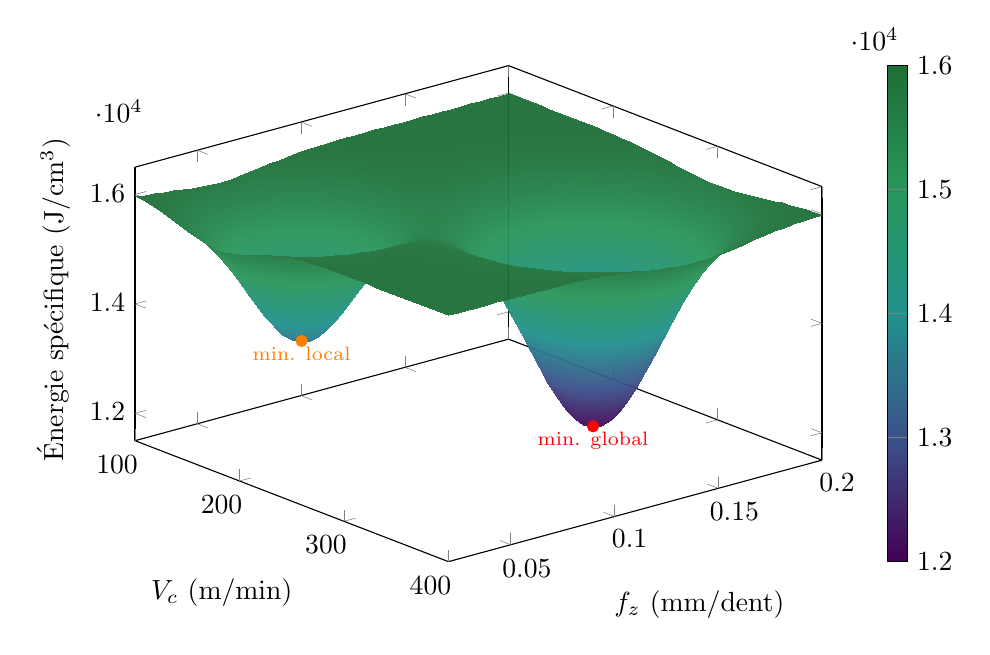
\begin{tikzpicture}
\begin{axis}[
  width=0.85\linewidth, height=0.65\linewidth,
  view={50}{30},
  y tick label style={/pgf/number format/fixed},
  xlabel={$V_c$ (m/min)},
  ylabel={$f_z$ (mm/dent)},
  zlabel={Énergie spécifique (J/cm$^3$)},
  domain=100:400, y domain=0.02:0.20,
  samples=40, samples y=40,
  zmin=1.15e4, zmax=1.65e4,
  colormap={viridisfonce}{rgb255=(68,1,84) rgb255=(59,82,139) rgb255=(33,145,140) rgb255=(40,150,90) rgb255=(30,110,55)},
  colorbar,
  colorbar style={width=0.25cm},
  declare function={
    Wc(\x,\y) = 16000
      - 4000*exp(-( ((\x-300)/60)^2 + ((\y-0.14)/0.035)^2 ))
      - 2500*exp(-( ((\x-180)/50)^2 + ((\y-0.06)/0.030)^2 ));
  },
]
  % Surface
  \addplot3[surf, shader=interp, opacity=0.95] {Wc(x,y)};

  % Minimum global
  \addplot3[only marks, mark=*, mark size=2pt, red]
    coordinates {(300,0.14,12000)}
    node[below, font=\scriptsize, inner sep=2pt] {min. global};

  % Minimum local
  \addplot3[only marks, mark=*, mark size=2pt, orange]
    coordinates {(180,0.06,13500)}
    node[below, font=\scriptsize, inner sep=2pt] {min. local};
\end{axis}
\end{tikzpicture}